% Bu doküman IEEE Türkiye tarafından düzenlenen TUAC için oluşturulmuş taslaktır. Yalnızca içeriklerin değiştirilmesi gerekmekte, dosya ayarlarında değişiklik yapılmaması önerilmektedir.

% Belgenin formatı değiştirilmemelidir.
\documentclass[conference, a4paper]{IEEEtran}
\IEEEoverridecommandlockouts

% Türkçe karakterler için:
\usepackage[turkish]{babel}
\usepackage[utf8]{inputenc} % Kullanılan kodlamaya göre "utf8" yerine "latin5" de tercih edilebilir.
\usepackage[T1]{fontenc}


\usepackage{float}

% ".jpeg" ve ".png" gibi görüntülerin belgede kullanılması için:
\usepackage[pdftex]{graphicx}

% Tablolarda birden fazla satır kullanılabilmesi için:
\usepackage{multirow}

% Referansların verilmesi ve numaralandırılması için:
\usepackage{cite}

% Matematiksel gösterimler için:
\usepackage[cmex10]{amsmath}

% SI ölçü birimlerinin kullanılabilmesi için:
\usepackage{siunitx}

% Matrisler ve diğer dizilerin kullanılabilmesi için:
\usepackage{array}

% Alt şekillerin değiştirilip, referans edilebilmesi için:
\usepackage[caption=false,lofdepth,lotdepth]{subfig}

% Kısaltmalar için:
\usepackage{acronym}
% Örnek Kısaltma
\acrodef{TUAC}{The Undergraduate Academic Conference}

% Hatalı hecelemeler örnekteki gibi düzeltilebilir
\hyphenation{op-tical net-works semi-conduc-tor}

\setlength{\textfloatsep}{5pt}

\AtBeginDocument{%
	\renewcommand\tablename{TABLO}
}

\AtBeginDocument{%
	\renewcommand\abstractname{Abstract}
}

\begin{document}
% Bildiri başlığı
% Daha iyi bir biçimlendirme için \linebreak komutu satır atlamak için kullanılabilir
\title{MQTT Protokolünde Şifreli Mesajların OTEL Tracing ve Zipkin Metrik Analizi: Algoritmaların Karşılaştırılması}

% Yazar isimleri ve bağlantıları
% Üç farklı yazar için çoklu sütun kullanılmalıdır
\author{\IEEEauthorblockN{Emre Erkan}
\IEEEauthorblockA{Bilgisayar Mühendisliği\\
Pamukkale Üniversitesi\\
Denizli, Türkiye\\
eerkan13@posta.pau.edu.tr}}

	% Başlığın yazdırılması
	\maketitle
	
	\begin{ozet}
		Bu çalışma, MQTT protokolü üzerinde şifreli mesaj iletimini ele almakta ve bu şifreli mesajların OTEL protokolü ile izlenmesi ile Zipkin üzerinde çeşitli metriklerin analizini sunmaktadır. AES, Blowfish, Camellia, CAST5, IDEA, SEED, TripleDES gibi çeşitli şifreleme algoritmaları, 16, 32, 64, 128, 256, 512, 1024, 2048 uzunluğundaki veriler üzerinde 1000’er  örnek üzerinde test edilmiştir. Elde edilen sonuçlar, her algoritmanın performansını, gecikme süresi, şifreleme/deşifreleme süreleri ve bellek tüketimi açısından ayrıntılı bir şekilde değerlendirmektedir. Bu analiz, güvenli ve etkin bir iletişim için algoritma seçiminde rehberlik sağlamayı amaçlamaktadır.
		%\boldmath
	\end{ozet}
	\begin{IEEEanahtar}
		mqtt, şifreli mesaj iletimi, otel protokolü, zipkin metrik analizi, şifreleme algoritmaları, iot
	\end{IEEEanahtar}
	
	\begin{abstract}
		This study, addresses encrypted message transmission on the MQTT protocol, presenting an analysis of various metrics on Zipkin through the monitoring of these encrypted messages using the OTEL protocol. Various encryption algorithms such as AES, Blowfish, Camellia, CAST5, IDEA, SEED, and TripleDES have been tested on data lengths of 16, 32, 64, 128, 256, 512, 1024, and 2048 in 1000 examples each. The results obtained comprehensively evaluate the performance of each algorithm in terms of latency, encryption/decryption times, and memory consumption. This analysis aims to provide guidance in selecting algorithms for secure and efficient communication.
	\end{abstract}
	\begin{IEEEkeywords}
		mqtt, encrypted message transmission, OTEL protocol, zipkin metric analysis, encryption algorithms, iot
	\end{IEEEkeywords}
	
	\IEEEpeerreviewmaketitle
	
	\IEEEpubidadjcol
	
	
	\section{G{\footnotesize İ}r{\footnotesize İ}ş}
	
	Dijital iletişimde güvenlik, veri bütünlüğü ve gizliliği sağlamak son derece kritik bir konudur. Bu bağlamda, MQTT (Message Queuing Telemetry Transport) protokolü, hafif ve etkili iletişim sağlama yeteneği ile nesnelerin interneti (IoT) ve diğer uygulama alanlarında geniş bir kullanım bulmuştur. Bu protokolün kullanımında, özellikle hassas verilerin iletilmesi durumunda, şifreleme önemli bir rol oynamaktadır.

    Bu çalışma, MQTT protokolünde şifreli mesajların iletimi üzerine odaklanmaktadır. Şifreli mesajların güvenli bir şekilde iletilmesi, veri bütünlüğünün sağlanması ve gizliliğin korunması, günümüzdeki birçok uygulama senaryosu için kritik öneme sahiptir. Bununla birlikte, şifreleme kullanımının getirdiği ek yükler ve performans etkileri, özellikle kaynak kısıtlı cihazlar ve ağlar için önemli bir konudur.

    Bu bağlamda, MQTT protokolünde kullanılan şifreleme algoritmalarının performansını değerlendirmek amacıyla gerçekleştirilen bu çalışma, şifreli mesajların OTEL (OpenTelemetry) protokolü ile izlenmesi ve Zipkin üzerinde çeşitli metriklerin analizini sunmaktadır. AES, Blowfish, Camellia, CAST5, IDEA, SEED, TripleDES gibi farklı şifreleme algoritmaları, değişen veri uzunlukları üzerinde test edilmiş ve bu algoritmaların performansı gecikme (latency), şifreleme/deşifreleme süreleri ve bellek tüketimi açısından detaylı bir şekilde incelenmiştir. Elde edilen sonuçlar, MQTT protokolünde şifreli iletişimin etkin bir şekilde yönetilebilmesi için önemli bir kılavuz sunmaktadır.
 
	\section{{\footnotesize İ}lg{\footnotesize İ}l{\footnotesize İ} {\footnotesize Ç}alışmalar}

    Panahi ve diğerleri (Panahi, P., Bayılmış, C., Çavuşoğlu, U., 2021) günümüzdeki tüm akıllı cihazların buluta bağlanma kabiliyetini ve bu sayede verilere her an her yerden erişilebilirliğin önemini vurgular. IoT ağı, veri transferinin yoğunluğu nedeniyle güvenli mekanizmaların uygulanma gerekliliğini ortaya koyar. Makale, sınırlı kaynaklara sahip IoT düğümleri için maliyet etkin ve verimli bir çözüm olan hafif blok şifrelerinin performansını değerlendirir. Raspberry Pi 3 ve Arduino Mega 2560 ile gerçekleştirilen simülasyonlar, IoT geliştiricilerine enerji ve bellek kullanımını göz önüne alarak güvenli bir ağ kurmak için doğru platformu ve şifreleme algoritmasını seçme konusunda rehberlik eder \cite{paper1}.

    Gunathilake ve diğerleri (Gunathilake, Buchanan ve Asif, 2019) hafif Şifreleme (LWC) algoritmalarının akıllı IoT cihazlarında uygulanması, özellikle de Long-Range Wide Area Network (LoRaWAN) teknolojisinin performansı ele alınmıştır. LoRaWAN, Low-Power Wide Area Network (LPWAN) teknolojisi için iletişim protokolünü tanımlayan bir açık standarttır \cite{paper2}.

    Shah ve diğerleri (Shah, Arora ve Adhvaryu, 2020) gömülü sistemlerde kullanılan geleneksel kriptografik algoritmaların, fiziksel boyut, işleme gereksinimleri ve bellek kısıtlamaları gibi sorunlarla başa çıkma konusundaki zorlukları ele alan bir araştırma makalesi bulunmaktadır. Bu makale, AES (Gelişmiş Şifreleme Standardı), SHA-256 (Güvenli Karma Algoritması) ve RSA/Elliptic Curve gibi yaygın kullanılan algoritmaların, düşük güç tüketimli cihazlar, sensör ağları ve sağlık uygulamaları gibi kaynak kısıtlı ortamlarda etkisiz kalabileceğini vurgulamaktadır \cite{paper3}.

    Gunathilake ve diğerleri (Gunathilake, Al-Dubai ve Buchana, 2020) hafif kriptografinin IoT platformlarına uygunluğunu vurgular. Geleneksel yöntemlerin ağırlıklarından kaçınarak yeni algoritmaların geliştirilmesi, gelişmiş IoT tehditlerine karşı direncin artırılmasını amaçlar. Çalışma, bu alanda literatür eksikliğini kapatmayı hedefler, gelişmeleri özetler ve gelecekteki geliştirmelere odaklanır \cite{paper4}.

    Al-Odat ve diğerleri (Al-Odat, Al-Qtiemat ve Khan, 2020) büyük veri ve IoT uygulamaları için bir hafif kriptografi karma fonksiyonunu tanıtır. Önerilen tasarım, S-Box, lineer dönüşüm ve bit permütasyon işlevlerini kullanarak güvenli ve hızlı bir hafif kriptografi protokolü sağlar. Tasarım, hız, bellek ve güç tüketimi açısından diğer hafif protokollerden üstün performans sergilemektedir \cite{paper5}.

    Bagla ve diğerleri (Bagla, Sharma, Mishra, Tripathi, Dumka ve Pandey, 2023) IoT ve bulut sistemlerinde güvenliği artırmak amacıyla örgü tabanlı kriptografiyi tanıtır. Örgü tabanlı şifreleme avantajları, geleneksel RSA ve eliptik eğri kriptografisiyle karşılaştırılarak incelenir. Ayrıca, IoT ve bulut sistemleri için özel olarak geliştirilen "Örgü Tabanlı Güvenli Veri Birleştirme" yaklaşımını sunar. Çalışma, veri şifreleme, birleştirme, deşifreleme ve sınırlı kaynaklı cihazlarda uygulama gibi çeşitli yönleri kapsar \cite{paper6}.

    Madavi ve diğerleri (Madavi, Sowjanya ve Patwari, 2023) IoT cihazlarının ürettiği verilerin güvenliği için Hafif Kriptografi (LWC) tekniklerini önermektedir. Öne çıkan yöntem, sağlık giyilebilir IoT cihazlarından elde edilen verileri tek bir düz metin içinde birleştirip şifreleyerek gizlilik ve güvenlik sağlamayı amaçlamaktadır. Önerilen yöntem, şifreleme ve deşifre sürelerini azaltarak daha iyi bir performans sunmaktadır \cite{paper7}.

    Nouha Oualha ve diğerleri (Oualha, Nouha, ve Kim Thuat Nguyen, 2016) "Internet of Things için Hafif Özellik Tabanlı Şifreleme" başlıklı çalışmada, yazarlar, etkili ön hesaplama tekniklerini kullanarak CP-ABE şemasını önermektedirler. Genellikle aşırı miktarda kriptografik işlem gerektiren set çiftlerini önceden hesaplamak ve sıkça kullanılan kriptografik operasyonlarla toplanan set çiftlerini önbelleğe almayı amaçlamaktadır. Üreteç tabanlı ön hesaplama teknikleri, genellikle donanım cihazları veya güvenilir otoriteler tarafından gerçekleştirilen üreteç ön işleme algoritmalarına dayanmaktadır. Bu ön hesaplama teknikleri, CP-ABE şifreleme maliyetini azaltırken, aynı zamanda orijinal şemadan daha az hesaplama gücü ve enerji tüketimi gerektiren bir yaklaşım sunmaktadır \cite{paper8}.

    Yijun Maoa  ve diğerleri (Mao, Yijun, Jin Li, Min-Rong Chen, Jianan Liu, Congge Xie ve Yiju Zhan, 2016) IoT'da veri iletimini korumak için yeni bir FSFIBE tekniği önermişlerdir. FSFIBE tekniği, rastgele oraçları içermeyen tam modelde güvenlidir. FSFIBE tekniği, sıkı güvenlik azaltma ve O(1) sabit boyutta genel parametrelere sahiptir. FSFIBE tekniği, hata toleransı özelliğini sunmaktadır \cite{paper9}.

    Fagen Li ve diğerleri (Li, Fagen, Zhaohui Zheng ve Chunhua Jin., 2016) kaynak kısıtlı cihazlardan bir sunucuya güvenli iletişim için heterojen bir halka imzaşifreleme tekniği önermektedir. Heterojen halka imzaşifreleme tekniği, IBC ortamında göndereni PKI etki alanındaki bir alıcıya mesaj göndermeye yetkilendirir. Teknik aynı anda gizlilik, bütünlük, kimlik doğrulama, reddedilememe ve anonimliği mantıklı bir tek adımda sağlamaktadır \cite{paper10}.
    
    Kun-Lin Tsai ve diğerleri (Tsai, Kun-Lin, Yi-Li Huang, Fang-Yie Leu ve Ilsun You, 2016) üçüncü taraf tabanlı çoklu anahtar değişim protokolünü önermiş ve eliptik eğri şifreleme ve deşifreleme kullanmışlardır. Bu protokol, Replay saldırısı, Eavesdropping saldırısı, Known-key saldırısı, Impersonation saldırısı, Forgery saldırısına karşı güvenlidir \cite{paper11}.
 
	\section{Geliştirilen Model}
    Bu bölümde, geliştirilen sistemin ayrıntılı bir teknik incelemesi sunulacaktır. Yazılım entegrasyonundan, iletişim protokollerine ve genel sistem mimarisine kadar her bir unsura geniş bir perspektiften yaklaşılacaktır. 
	
	\subsection{Sistem Mimarisi}

    Geliştirilen modelin sistem mimarisi, şifreli mesaj üretiminden başlayarak çeşitli önemli bileşenleri içerir. İlk olarak, "Publisher" bileşeni, MQTT protokolü kullanarak şifrelenmiş mesajları üretir. Ardından, bu şifreli mesajlar "Gateway" bileşeni aracılığıyla iki ayrı MQTT brokerı arasında eşitlenir. Şifrelenmiş verilerin güvenli bir şekilde iletimi sağlanmış olur. Son aşamada ise, şifrelenmiş verileri alıp çözümleyen "Subscriber" bileşeni bulunmaktadır. Bu bileşen, orijinal veriyi elde ederek son kullanıcıya sunar. Bu süreç, güvenli ve etkili bir iletişimi temsil eder, bu da şifrelenmiş verilerin güvenli bir şekilde kaynak ve hedef arasında iletilmesini sağlar.

\begin{figure}[H]
    \centering
    \shorthandoff{=}  
    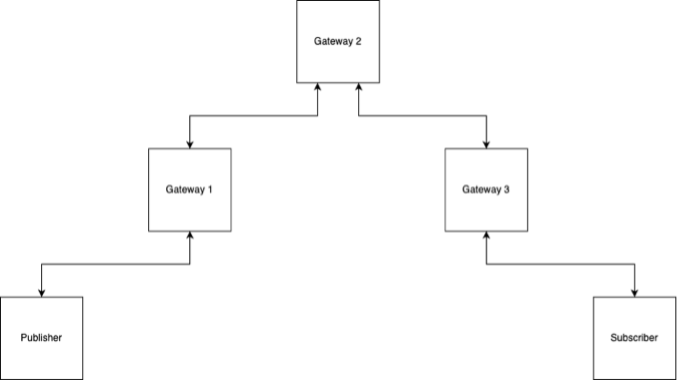
\includegraphics[scale=1.00]{fig1.png}
    \shorthandon{=} 
    \caption{Sistem mimarisi.}
    \label{sekil1}
\end{figure}

	\subsection{MQTT Protokolü}
    MQTT (Message Queuing Telemetry Transport), hafif, açık kaynaklı bir mesajlaşma protokolüdür ve özellikle düşük bant genişliğine sahip ve bağlantı kaynakları sınırlı cihazlar arasında güvenilir mesaj iletişimi sağlamak için tasarlanmıştır. Bu protokol, yayın/abone modelini temel alır ve genellikle IoT cihazları, sensör ağları ve dağıtık sistemlerde kullanılır.
    
    Geliştirilen projede, MQTT protokolü şifreli mesaj iletimi için temel iletişim protokolü olarak kullanılmaktadır. "Publisher" bileşeni, MQTT protokolünü kullanarak şifrelenmiş mesajları üretir ve bu mesajları belirli bir MQTT topic'ine gönderir. Ardından, bu şifreli mesajlar, "Gateway" bileşeni aracılığıyla farklı MQTT brokerları arasında eşitlenir. Bu sayede, güvenli bir şekilde şifrelenmiş veri, farklı brokerlar arasında güvenli bir iletim sağlanır. "Subscriber" bileşeni ise şifreli veriyi alır, çözümleme işlemi gerçekleştirir ve orijinal veriyi elde eder. MQTT protokolü, projede dağıtık ve güvenli iletişimi mümkün kılarak sistemin sağlıklı çalışmasını destekler.

    
\begin{figure}[H]
    \centering
    \shorthandoff{=}  
    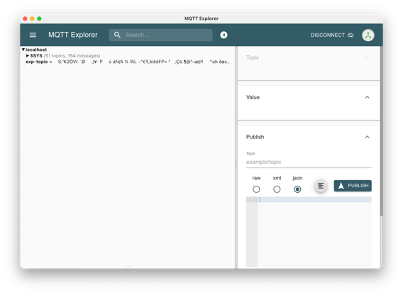
\includegraphics[scale=1.00]{fig2.png}
    \shorthandon{=} 
    \caption{MQTT broker’da bulunan şifrelenmiş mesaj.}
    \label{sekil2}
\end{figure}
	
	\subsection{Zipkin ve OTEL}
    Zipkin, mikroservis mimarisine sahip sistemlerdeki dağıtık uygulamalardan elde edilen verilerin izlenmesini ve analizini sağlayan bir açık kaynaklı bir izleme sistemidir. Zipkin, uygulamadaki farklı mikroservisler arasındaki bağlantıları ve veri akışını görselleştirmek için kullanılır. Bu sayede, uygulama içindeki performans sorunlarını tespit etmek ve iyileştirmeler yapmak daha kolay hale gelir.
    
    OpenTelemetry (OTEL), çeşitli programlama dilleri ve çerçeveler arasında uygulama performansını izlemek ve analiz etmek için kullanılan bir standarttır. OTEL, dağıtık uygulamalardan gelen verilerin toplanması, izlenmesi ve analiz edilmesi için genel bir çerçeve sağlar. Bu standart, farklı dil ve teknolojileri kullanan sistemler arasında tutarlı izleme ve analiz olanağı sağlar.
    
    Geliştirilen modelde, Zipkin ve OTEL protokolleri, MQTT üzerinden iletilen şifreli mesajların takibini ve analizini sağlamak amacıyla entegre edilmiştir. Zipkin, şifrelenmiş verilerin kaynağından hedefine kadar olan yolunu görselleştirmekte ve uygulamadaki her bir mikroservisin performansını izlemektedir. OTEL ise çeşitli dil ve teknolojiler kullanılarak geliştirilen bileşenlerden elde edilen metrik verilerin toplanmasını sağlar. Bu sayede, geliştirilen modelin performansını değerlendirmek ve olası iyileştirmeleri belirlemek için kapsamlı bir izleme ve analiz yapılmaktadır.

\begin{figure}[H]
    \centering
    \shorthandoff{=}  
    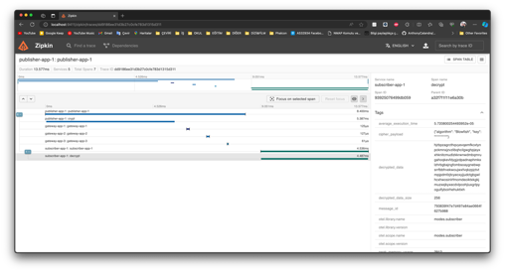
\includegraphics[scale=1.00]{fig3.png}
    \shorthandon{=} 
    \caption{İzlenilen mesajın zipkin görünümü.}
    \label{sekil3}
\end{figure}

 \subsection{Şifreleme Algoritmaları}
    AES, Rijndael algoritmasına dayanır ve 128, 192 veya 256 bit uzunluğunda anahtarlar kullanır. Blok başına 128 bit veri işler. SubBytes, ShiftRows, MixColumns ve AddRoundKey adlı dört temel işlem içerir. Bu sayede saldırılara karşı dirençli ve hızlı bir şifreleme sağlar.
 
    Blowfish, Feistel ağı yapısına dayanır ve değişken uzunluktaki anahtarları destekler. Bir turdaki işlemler arasında sırasıyla XOR, S-Box uygulaması, Permutasyon ve Substitution işlemleri bulunur. Esnek anahtar uzunlukları ve hızlı işleme yetenekleri nedeniyle tercih edilir.
    
    Camellia, Feistel ağı yapısına dayalı simetrik bir blok şifreleme algoritmasıdır. S-Box, Permutasyon ve anahtar eklemesi gibi işlemler içerir. Japon ve Güney Kore kriptografi standartları için kullanılır ve AES'e benzer güvenlik düzeyleri sağlar.

    CAST5, Carlisle Adams ve Stafford Tavares tarafından geliştirilen bir simetrik blok şifreleme algoritmasıdır. Feistel şifreleme yapısını kullanır ve anahtar uzunluğu değiştirilebilir. Veri bloklarını şifrelemek için S-Box ve anahtar eklemesi gibi işlemleri içerir.

    IDEA, 64-bit blokları şifrelemek ve deşifre etmek için kullanılan bir simetrik anahtarlı şifreleme algoritmasıdır. 128 bit uzunluğundaki anahtarları destekler. Permutasyon, XOR ve modüler aritmetik gibi işlemler içerir. Güvenilir ve hızlı bir şifreleme sağlar.

    SEED, Güney Kore'nin geliştirdiği bir blok şifreleme algoritmasıdır. 128 bit uzunluğundaki anahtarları kullanır. Feistel ağı yapısını benimser ve XOR, Permutasyon ve Substitution gibi işlemleri içerir. Hızlı ve güvenilir bir şifreleme sağlar.

    TripleDES, DES algoritmasının üç kere uygulanmasıyla oluşan bir şifreleme yöntemidir. Anahtar uzunluğu 168 bit olabilir. DES'e dayalı olması, daha güvenilir ve dayanıklı bir şifreleme sağlar. Feistel ağı yapısını üç katmanlı olarak kullanır.

\subsection{Algoritmaların Karşılaştırılması}

    \begin{figure}[H]
    \centering
    \shorthandoff{=}  
    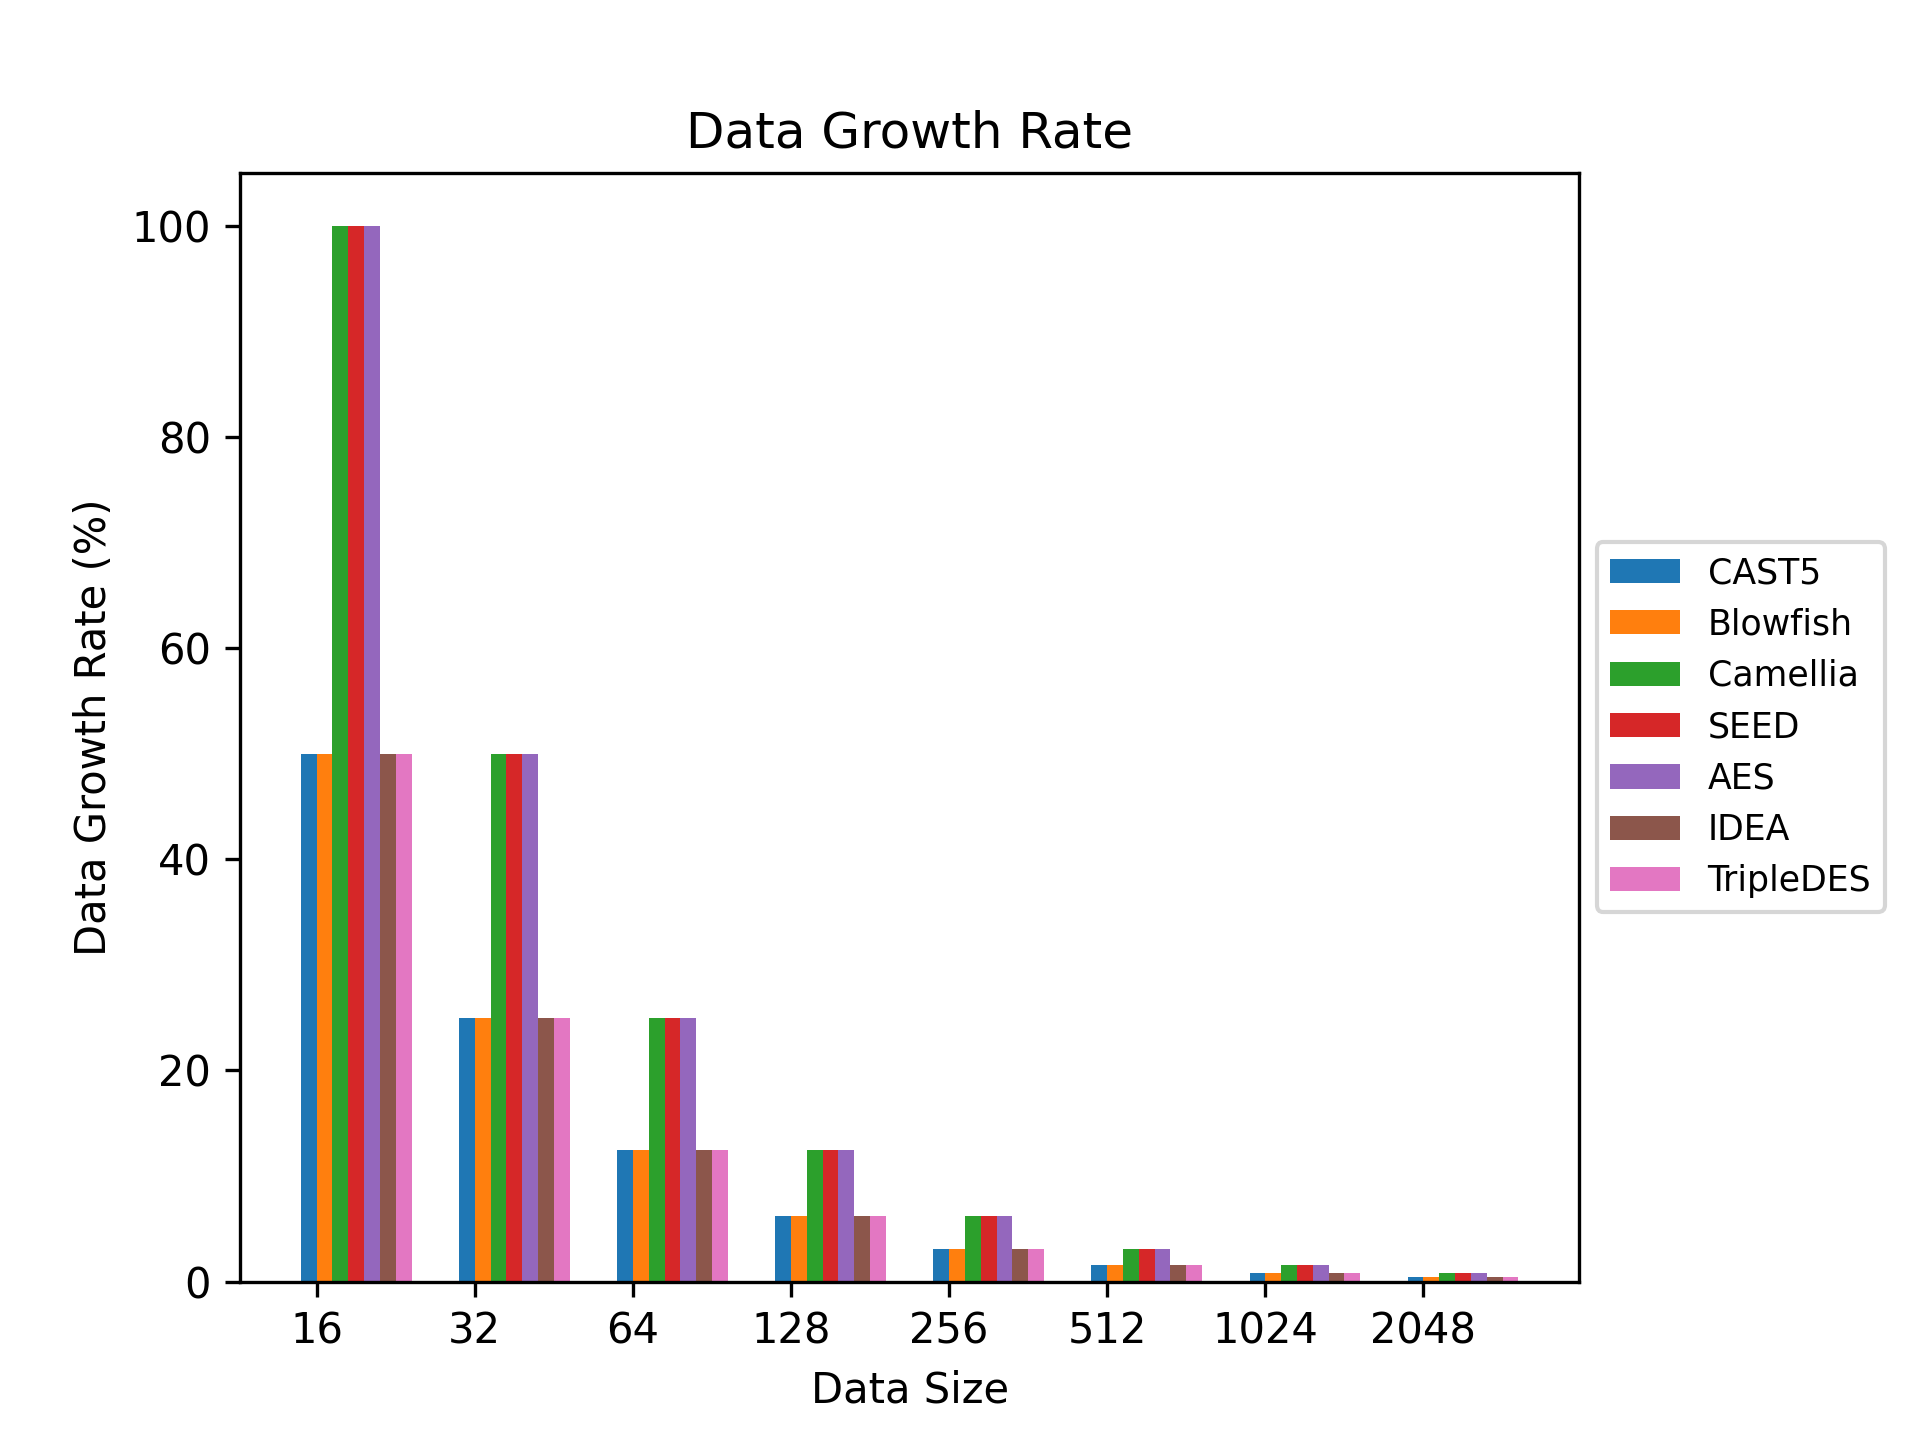
\includegraphics[scale=0.52]{fig4.png}
    \shorthandon{=} 
    \caption{Şifrelendikten sonra verinin büyüme oranı.}
    \label{sekil4}
    \end{figure}

    \begin{table}[h]
        \centering
        \caption{\textsc{Veri büyüme oranı}}
        \label{tablo1}
        \begin{tabular}{|c|c|}
            \hline
                Veri Boyutu & Algoritmalar sırasıyla en düşükten en yükseğe doğru \\
            \hline
            16 & Blowfish, TripleDES, CAST5, IDEA, SEED, Camellia, AES \\
            \hline
            32 & Blowfish, TripleDES, CAST5, IDEA, SEED, Camellia, AES \\
            \hline
            64 & Blowfish, TripleDES, CAST5, IDEA, SEED, Camellia, AES \\
            \hline
            128 & Blowfish, TripleDES, CAST5, IDEA, SEED, Camellia, AES \\
            \hline
            256 & Blowfish, TripleDES, CAST5, IDEA, SEED, Camellia, AES \\
            \hline
            512 & Blowfish, TripleDES, CAST5, IDEA, SEED, Camellia, AES \\
            \hline
            1024 & Blowfish, TripleDES, CAST5, IDEA, SEED, Camellia, AES \\
            \hline
            2048 & Blowfish, TripleDES, CAST5, IDEA, SEED, Camellia, AES \\
            \hline
        \end{tabular}
    \end{table}

    Küçük veri boyutlarında, Blowfish, TripleDES ve CAST5 algoritmaları, şifreleme işlemi sonucunda veri boyutunu daha etkin bir şekilde küçük tutmaktadır. Bu algoritmalar, düşük veri büyüme oranlarıyla öne çıkar. Bu özellikleri, veri güvenliğini korurken aynı zamanda kaynakları daha verimli bant genişliği kullanma avantajı sunmaktadır.

    \begin{figure}[H]
    \centering
    \shorthandoff{=}  
    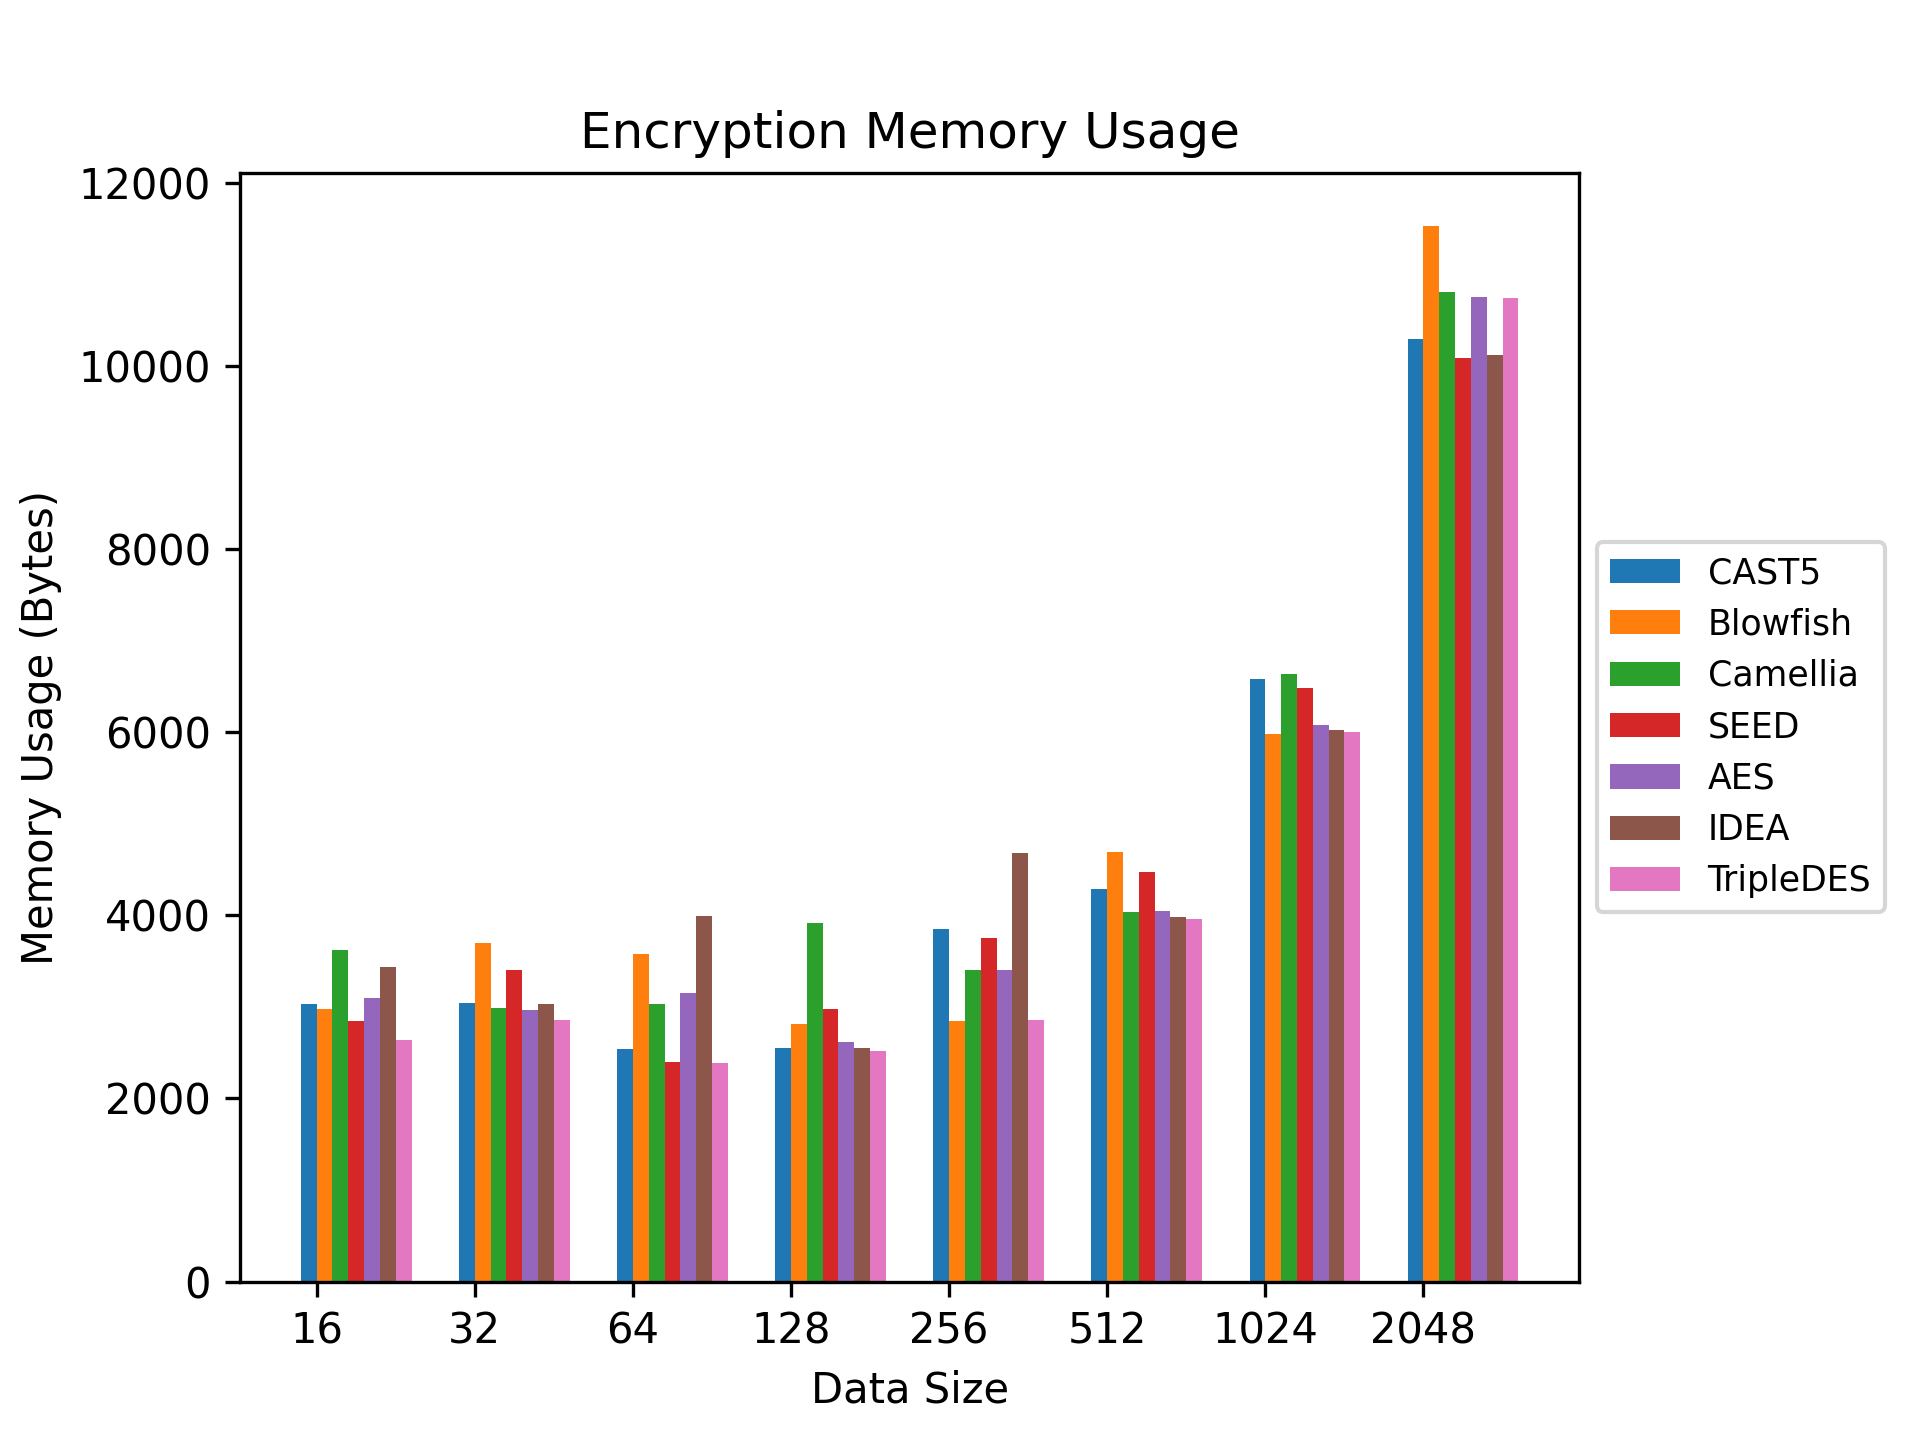
\includegraphics[scale=0.52]{fig5.png}
    \shorthandon{=} 
    \caption{Şifreleme bellek kullanımı.}
    \label{sekil5}
    \end{figure}

    \begin{table}[h]
        \centering
        \caption{\textsc{Şifreleme bellek kullanımı}}
        \label{tablo2}
        \begin{tabular}{|c|c|}
            \hline
                Veri Boyutu & Algoritmalar sırasıyla en düşükten en yükseğe doğru \\
            \hline
            16 & TripleDES, SEED, Blowfish, CAST5, AES, IDEA, Camellia \\
            \hline
            32 & TripleDES, AES, Camellia, IDEA, CAST5, SEED, Blowfish \\
            \hline
            64 & TripleDES, SEED, CAST5, Camellia, AES, Blowfish, IDEA \\
            \hline
            128 & TripleDES, CAST5, IDEA, AES, Blowfish, SEED, Camellia \\
            \hline
            256 & Blowfish, TripleDES, Camellia, AES, SEED, CAST5, IDEA \\
            \hline
            512 & TripleDES, IDEA, Camellia, AES, CAST5, SEED, Blowfish \\
            \hline
            1024 & Blowfish, TripleDES, IDEA, AES, SEED, CAST5, Camellia \\
            \hline
            2048 & SEED, IDEA, CAST5, TripleDES, AES, Camellia, Blowfish \\
            \hline
        \end{tabular}
    \end{table}

    Bellek tüketimi analizi sonuçlarına göre, veri boyutuna bağlı olarak TripleDES, SEED ve Blowfish algoritmalarının öne çıktığı gözlemlenmiştir. Özellikle düşük donanımlı cihazlar için bellek kullanımının kritik olduğu düşünüldüğünde, grafik ve tablo üzerindeki verilere dayanarak uygun algoritmanın seçimi önemli bir faktördür. Veri boyutuna özgü bellek performansını değerlendirerek, şifreleme algoritmalarının etkili bir şekilde seçilmesi, genel sistem performansını artırabilir ve kaynak kullanımını optimize edebilir.

    \begin{figure}[H]
    \centering
    \shorthandoff{=}  
    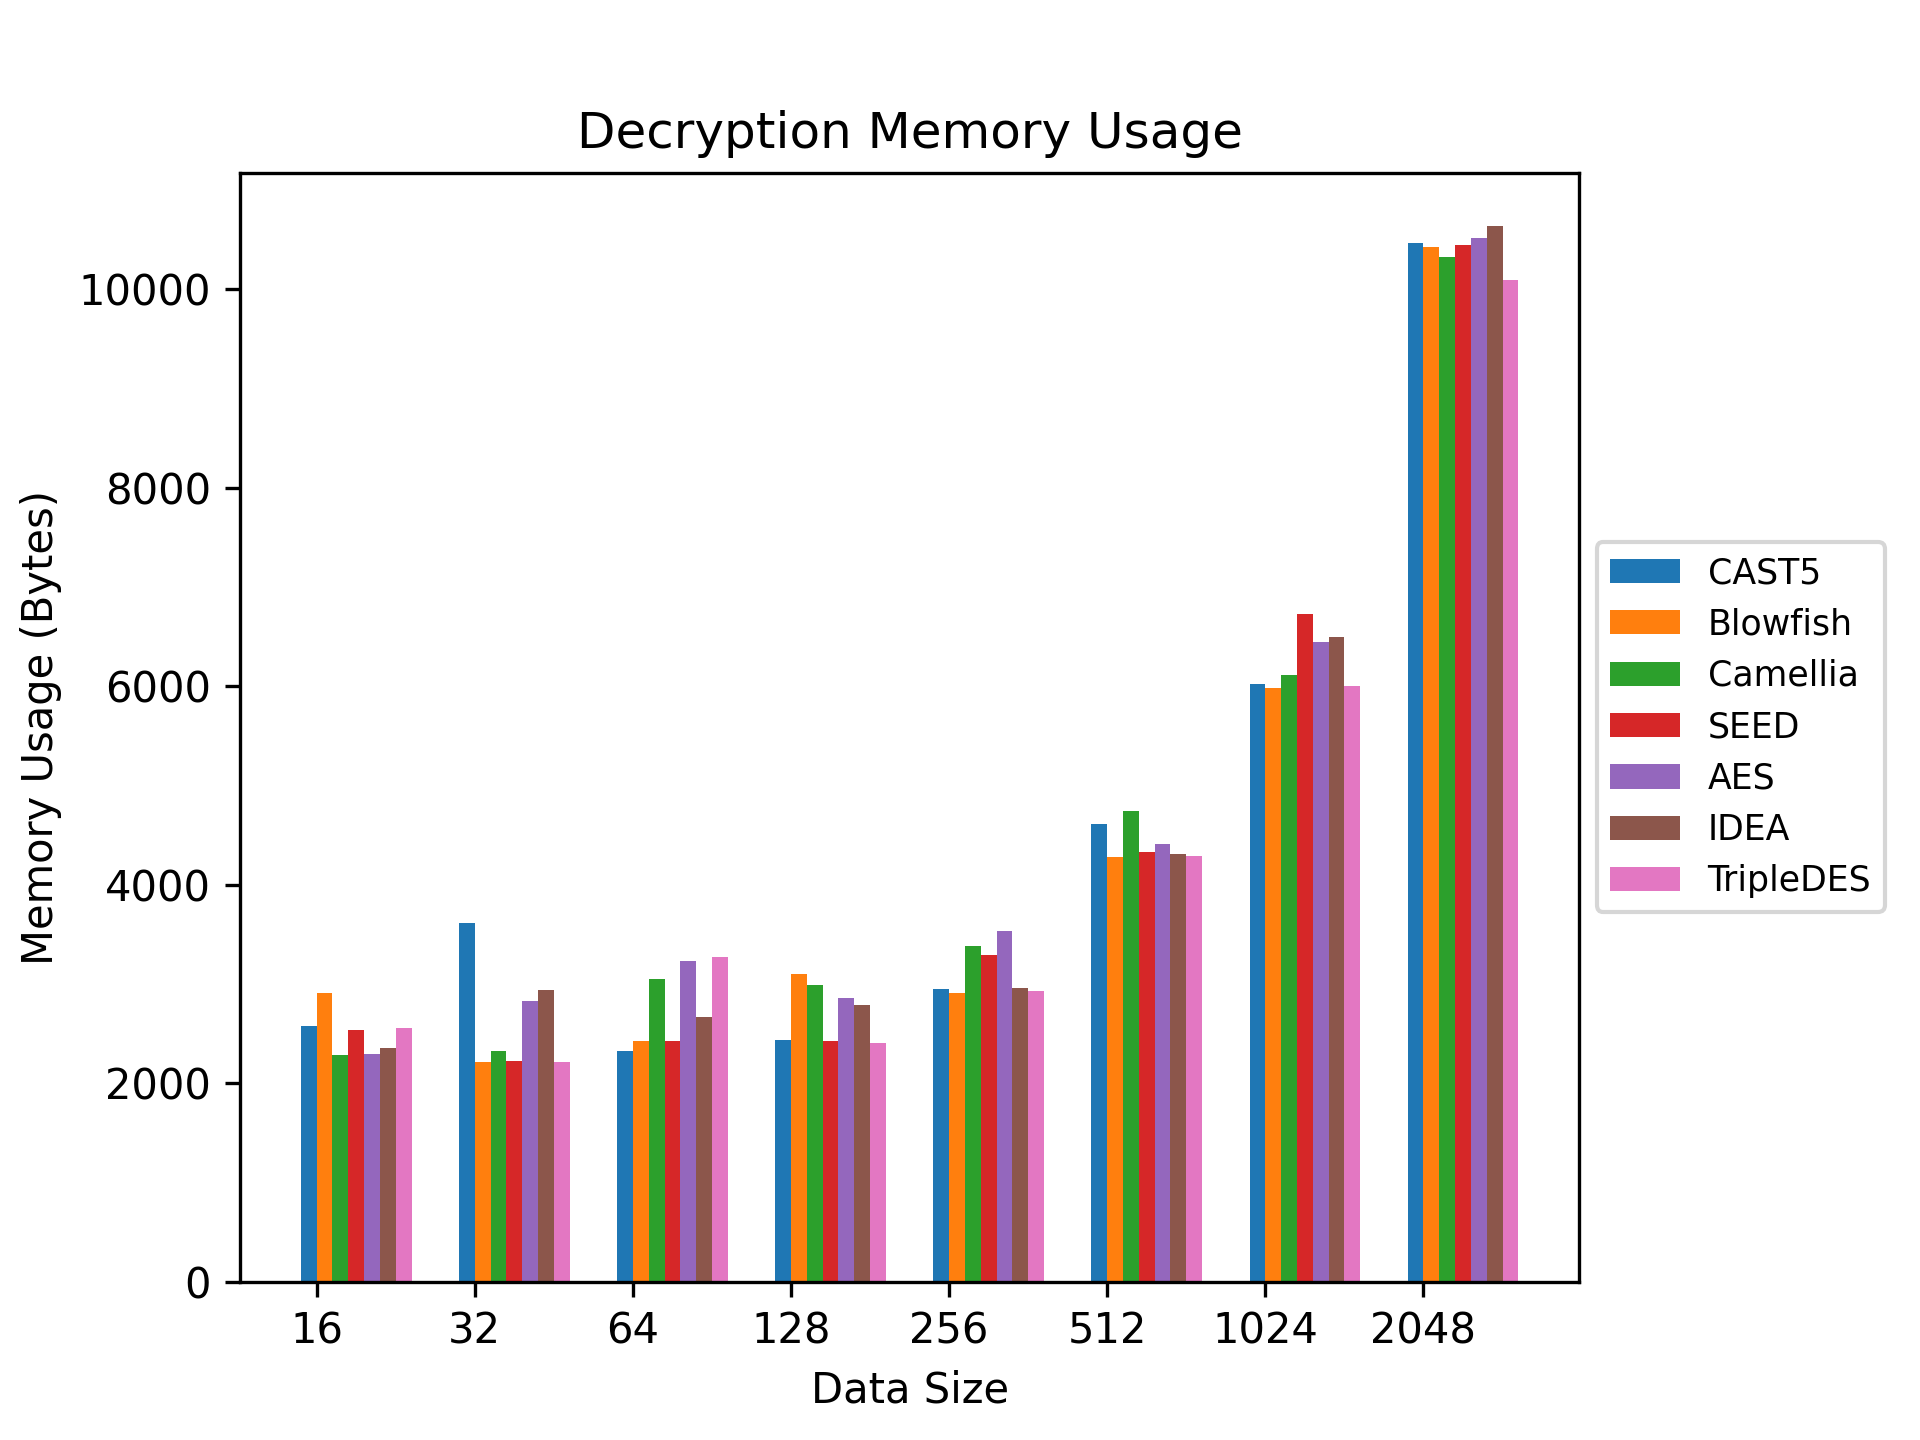
\includegraphics[scale=0.52]{fig6.png}
    \shorthandon{=} 
    \caption{Deşifreleme bellek kullanımı.}
    \label{sekil6}
    \end{figure}

    \begin{table}[h]
        \centering
        \caption{\textsc{Deşifreleme bellek kullanımı}}
        \label{tablo3}
        \begin{tabular}{|c|c|}
            \hline
                Veri Boyutu & Algoritmalar sırasıyla en düşükten en yükseğe doğru \\
            \hline
            16 & Camellia, AES, IDEA, SEED, TripleDES, CAST5, Blowfish \\
            \hline
            32 & TripleDES, Blowfish, SEED, Camellia, AES, IDEA, CAST5 \\
            \hline
            64 & CAST5, Blowfish, SEED, IDEA, Camellia, AES, TripleDES \\
            \hline
            128 & TripleDES, SEED, CAST5, IDEA, AES, Camellia, Blowfish \\
            \hline
            256 & Blowfish, TripleDES, CAST5, IDEA, SEED, Camellia, AES \\
            \hline
            512 & Blowfish, TripleDES, IDEA, SEED, AES, CAST5, Camellia \\
            \hline
            1024 & Blowfish, TripleDES, CAST5, Camellia, AES, IDEA, SEED \\
            \hline
            2048 & TripleDES, Camellia, Blowfish, SEED, CAST5, AES, IDEA \\
            \hline
        \end{tabular}
    \end{table}    

    Deşifreleme sürecinde, düşük veri boyutlarında SEED, TripleDES ve CAST5 algoritmaları belirgin bir performans sergilemektedir. Veri boyutları arttıkça Blowfish algoritması daha yüksek performans sağlamaktadır. Optimal performans için veri boyutuyla uyumlu şifreleme algoritmalarının seçilmesi önemlidir.

    \begin{figure}[H]
    \centering
    \shorthandoff{=}  
    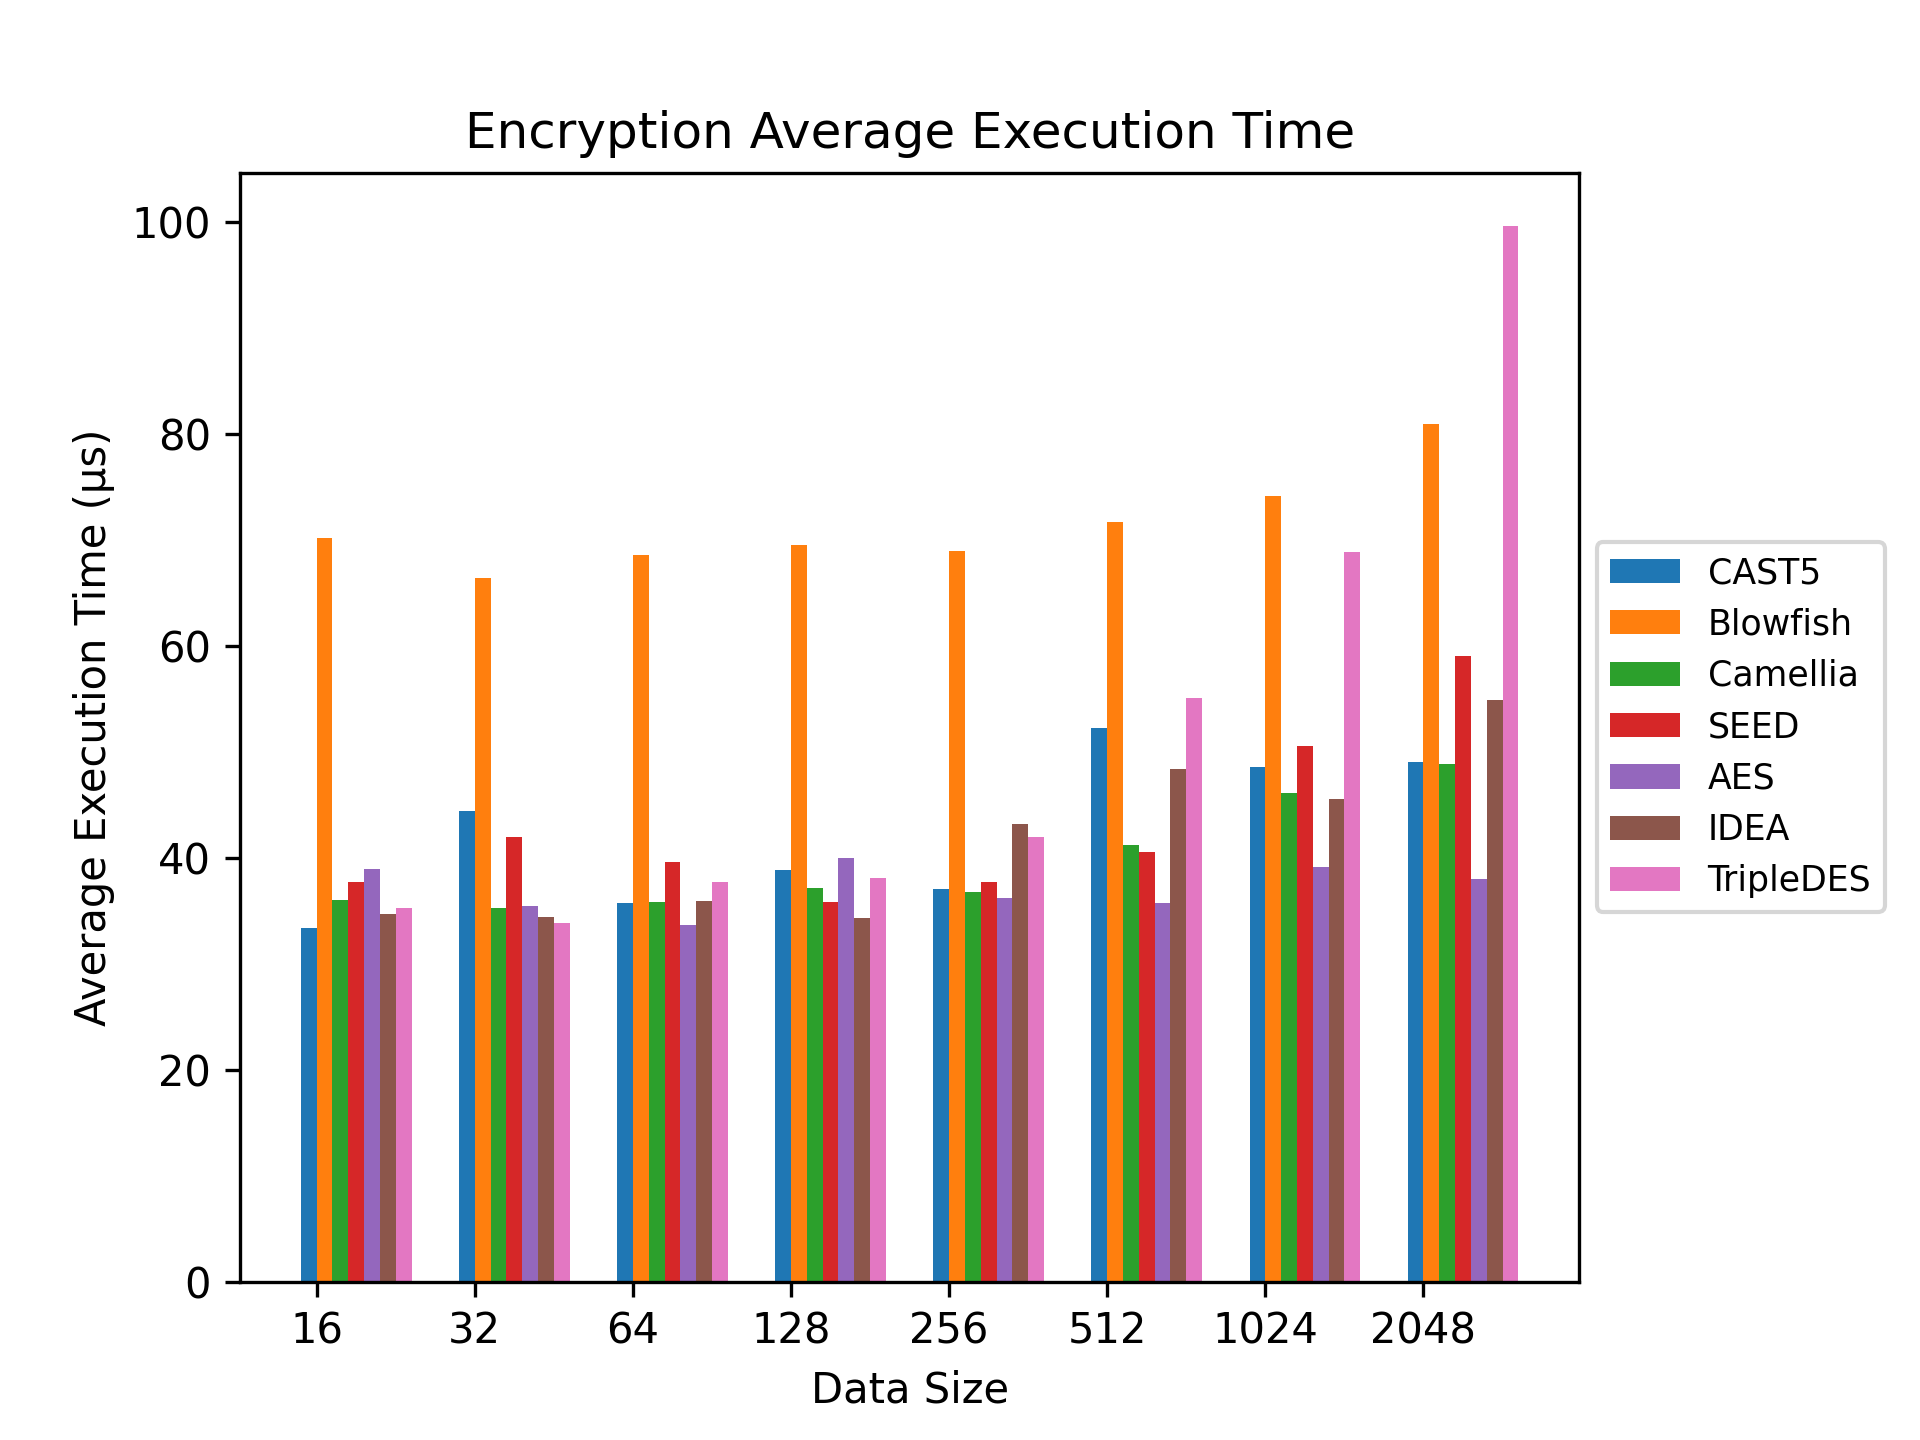
\includegraphics[scale=0.52]{fig7.png}
    \shorthandon{=} 
    \caption{Şifreleme süresi.}
    \label{sekil7}
    \end{figure}

    \begin{table}[h]
        \centering
        \caption{\textsc{Şifreleme süresi}}
        \label{tablo4}
        \begin{tabular}{|c|c|}
            \hline
                Veri Boyutu & Algoritmalar sırasıyla en düşükten en yükseğe doğru \\
            \hline
            16 & CAST5, IDEA, TripleDES, Camellia, SEED, AES, Blowfish \\
            \hline
            32 & TripleDES, IDEA, Camellia, AES, SEED, CAST5, Blowfish \\
            \hline
            64 & AES, CAST5, Camellia, IDEA, TripleDES, SEED, Blowfish \\
            \hline
            128 & IDEA, SEED, Camellia, TripleDES, CAST5, AES, Blowfish \\
            \hline
            256 & AES, Camellia, CAST5, SEED, TripleDES, IDEA, Blowfish \\
            \hline
            512 & AES, SEED, Camellia, IDEA, CAST5, TripleDES, Blowfish \\
            \hline
            1024 & AES, IDEA, Camellia, CAST5, SEED, TripleDES, Blowfish \\
            \hline
            2048 & AES, Camellia, CAST5, IDEA, SEED, Blowfish, TripleDES \\
            \hline
        \end{tabular}
    \end{table}    

    Şifreleme süresinde büyük veri boyutlarında AES algoritması ön plana çıkmaktadır. Çoğu durumda Blowfish algoritması düşük performans sağlamıştır.

    \begin{figure}[H]
    \centering
    \shorthandoff{=}  
    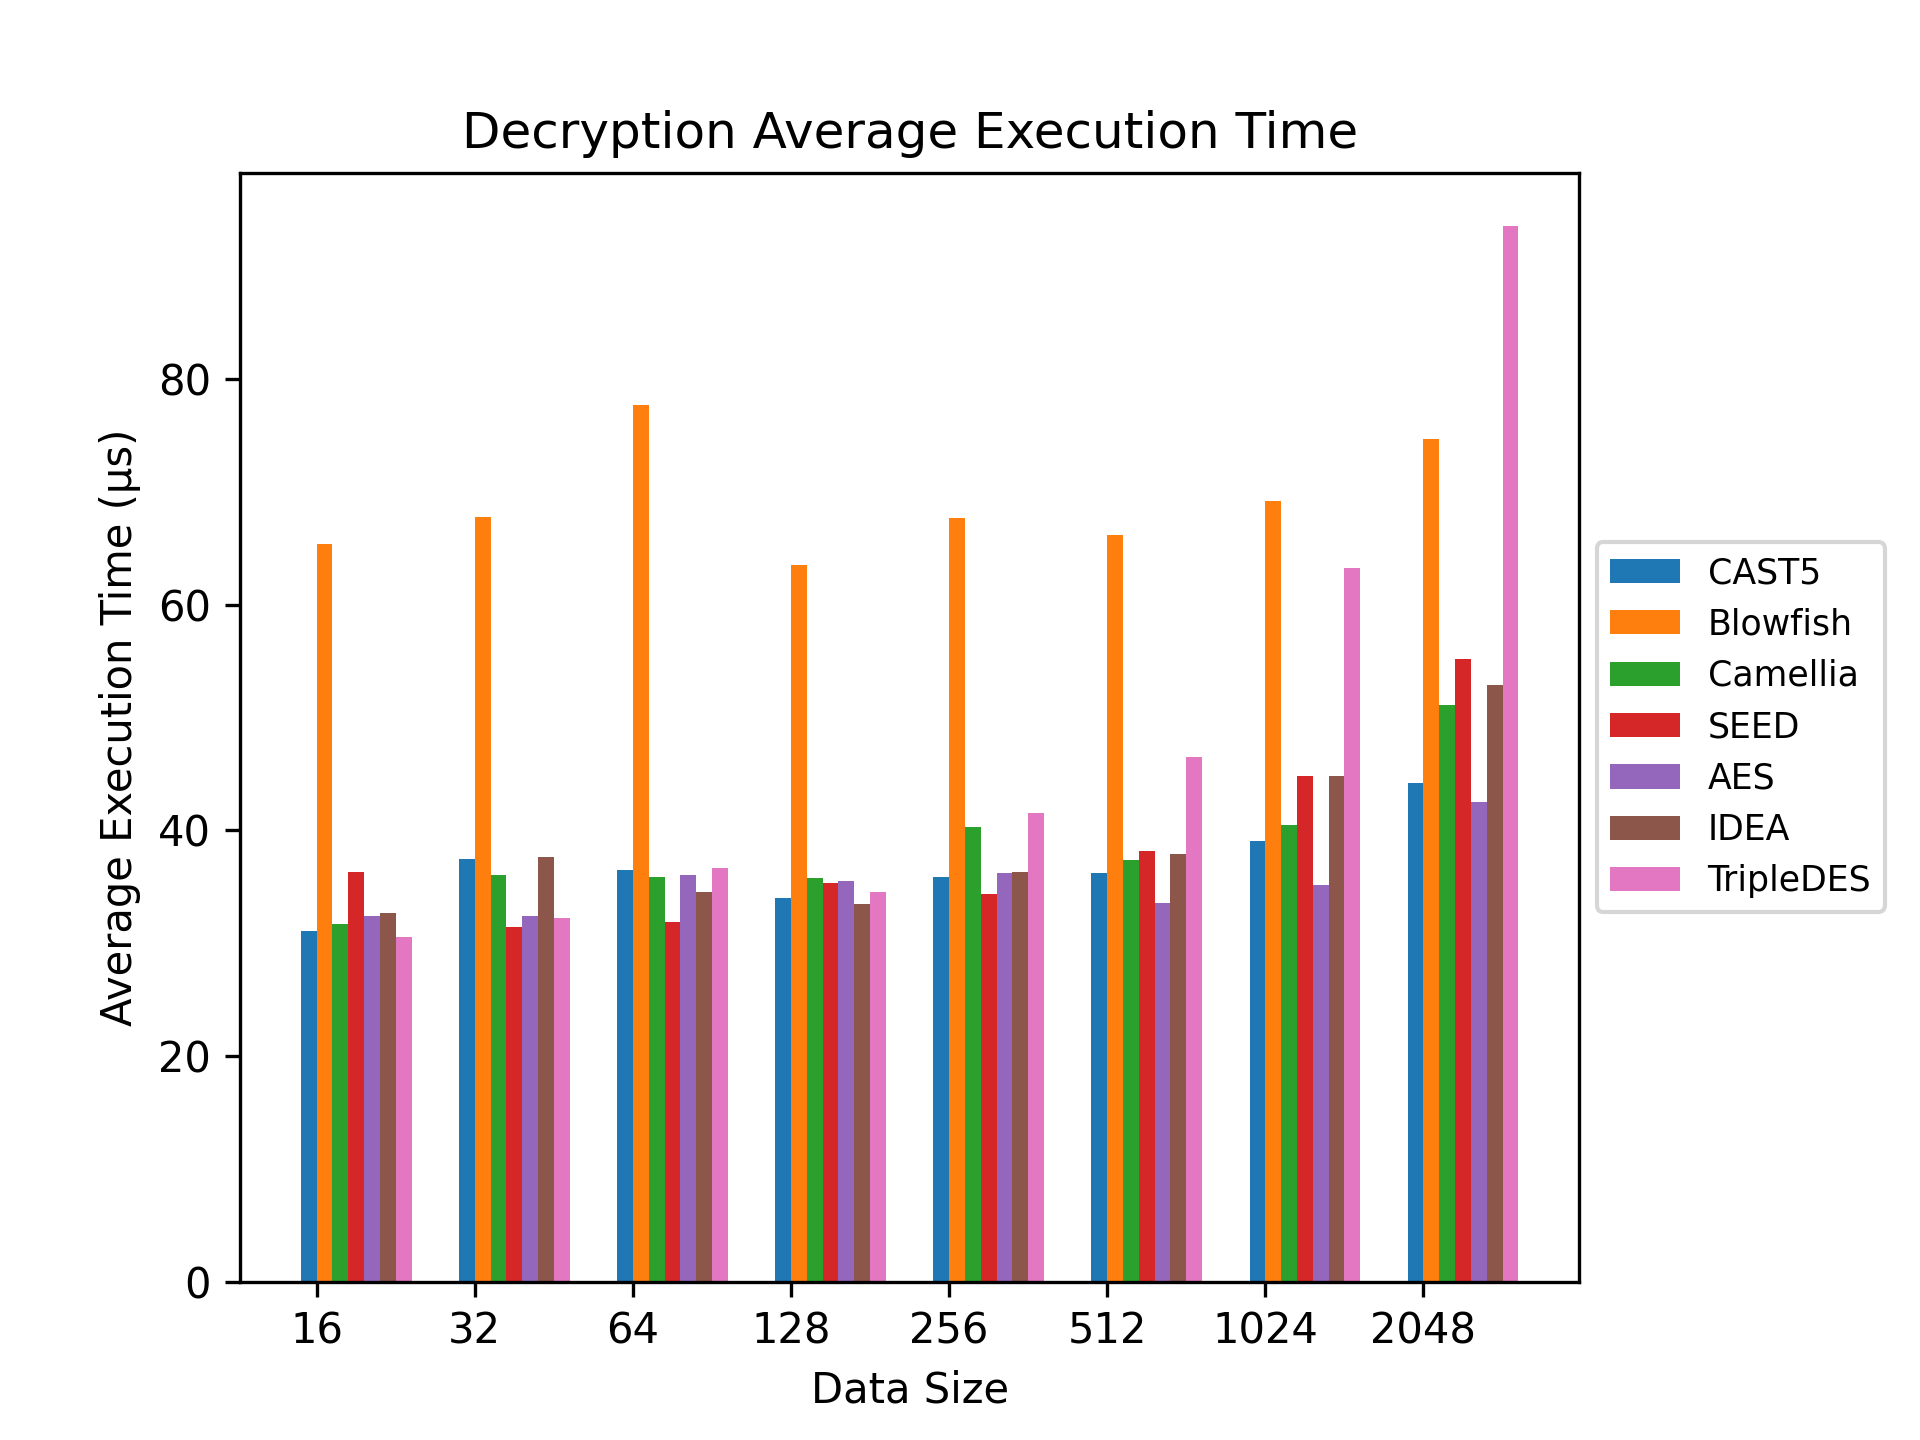
\includegraphics[scale=0.52]{fig8.png}
    \shorthandon{=} 
    \caption{Deşifreleme süresi.}
    \label{sekil8}
    \end{figure}

    \begin{table}[h]
        \centering
        \caption{\textsc{Deşifreleme süresi}}
        \label{tablo5}
        \begin{tabular}{|c|c|}
            \hline
                Veri Boyutu & Algoritmalar sırasıyla en düşükten en yükseğe doğru \\
            \hline
            16 & TripleDES, CAST5, Camellia, AES, IDEA, SEED, Blowfish \\
            \hline
            32 & SEED, TripleDES, AES, Camellia, CAST5, IDEA, Blowfish \\
            \hline
            64 & SEED, IDEA, Camellia, AES, CAST5, TripleDES, Blowfish \\
            \hline
            128 & IDEA, CAST5, TripleDES, SEED, AES, Camellia, Blowfish \\
            \hline
            256 & SEED, CAST5, AES, IDEA, Camellia, TripleDES, Blowfish \\
            \hline
            512 & AES, CAST5, Camellia, IDEA, SEED, TripleDES, Blowfish \\
            \hline
            1024 & AES, CAST5, Camellia, IDEA, SEED, TripleDES, Blowfish \\
            \hline
            2048 & AES, CAST5, Camellia, IDEA, SEED, Blowfish, TripleDES \\
            \hline
        \end{tabular}
    \end{table}    

    Deşifreleme süresi incelendiğinde düşük veri boyutlarında SEED ve TripleDES algoritması ön plana çıkmaktadır. Daha yüksek veri boyutlarında AES algoritması daha iyi performans sergilemiştir.

    \begin{figure}[H]
    \centering
    \shorthandoff{=}  
    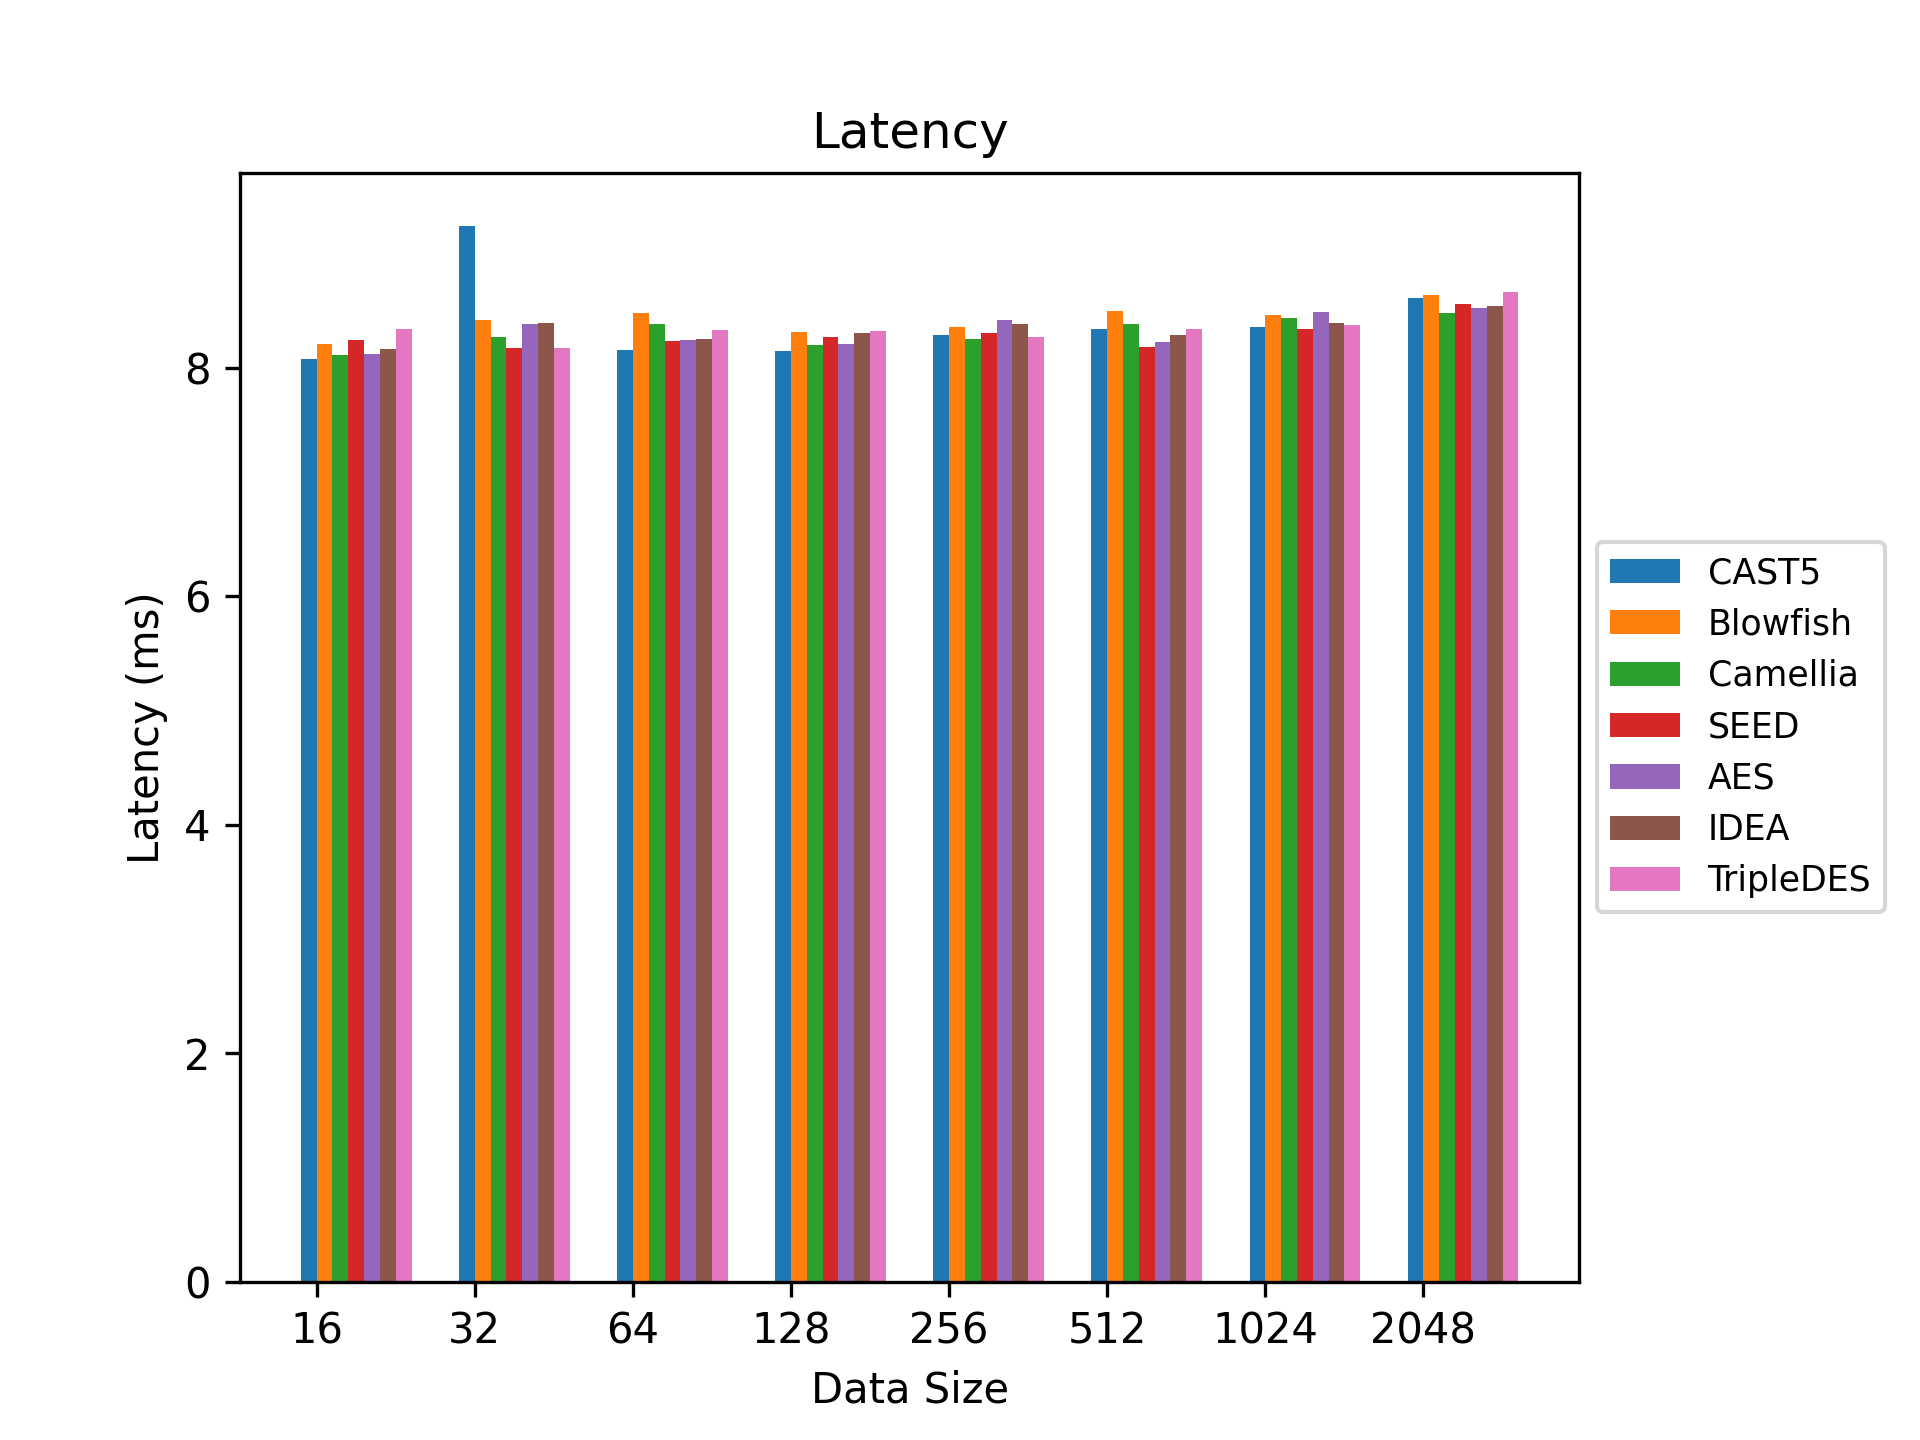
\includegraphics[scale=0.52]{fig9.png}
    \shorthandon{=} 
    \caption{Gecikme süresi.}
    \label{sekil9}
    \end{figure}

    \begin{table}[h]
        \centering
        \caption{\textsc{Gecikme süresi}}
        \label{tablo6}
        \begin{tabular}{|c|c|}
            \hline
                Veri Boyutu & Algoritmalar sırasıyla en düşükten en yükseğe doğru \\
            \hline
            16 & CAST5, Camellia, AES, IDEA, Blowfish, SEED, TripleDES \\
            \hline
            32 & SEED, TripleDES, Camellia, AES, IDEA, Blowfish, CAST5 \\
            \hline
            64 & CAST5, SEED, AES, IDEA, TripleDES, Camellia, Blowfish \\
            \hline
            128 & CAST5, Camellia, AES, SEED, IDEA, Blowfish, TripleDES \\
            \hline
            256 & Camellia, TripleDES, CAST5, SEED, Blowfish, IDEA, AES \\
            \hline
            512 & SEED, AES, IDEA, TripleDES, CAST5, Camellia, Blowfish \\
            \hline
            1024 & SEED, CAST5, TripleDES, IDEA, Camellia, Blowfish, AES \\
            \hline
            2048 & Camellia, AES, IDEA, SEED, CAST5, Blowfish, TripleDES \\
            \hline
        \end{tabular}
    \end{table}  

    Geliştirdiğimiz sistemde, gözlemlenen ortalama 8-9 ms arası gecikme süresi, algoritmanın etkisinin minimal olduğunu göstermektedir. Bu gecikme süresindeki artışın temel nedeni, MQTT broker ve Gateway programının çalışma yapısındadır. Algoritmanın hızlı ve etkili bir şekilde çalışmasına rağmen, bütün sistemin genel performansını etkileyen faktörler arasında MQTT broker ve Gateway programının belirgin bir rolü olduğu görülmektedir. Bu durum, sistem performansını daha fazla optimize etmek için bu bileşenlere odaklanmayı gerektirebilir.
    
    \section{Uygulamalar}
    Geliştirilen sistem, özellikle şifreleme odaklı özellikleri sayesinde çeşitli uygulama alanlarında güvenli iletişim ihtiyaçlarına hitap etmektedir. Bu sistem, Docker teknolojisi ve Python programlama dilinin entegrasyonu ile şifreli iletişim sağlamak amacıyla tasarlanmıştır.
    
    Öncelikle, Internet of Things (IoT) projelerinde bu sistem, IoT cihazları arasında güvenli ve şifrelenmiş veri iletimini destekleyerek endüstriyel IoT uygulamalarında, akıllı ev sistemlerinde ve medikal cihazlarda güvenlik sağlar. Hassas verilerin güvenli bir şekilde iletilmesi, bu tip projelerde kritik bir gerekliliktir.

    Merkezi olmayan veri senkronizasyonu, farklı MQTT broker'ları arasında şifreli veri eşitleme ihtiyacını karşılamaktadır. Bu, finansal projelerden enerji sektörüne kadar farklı alanlarda şifrelenmiş veri akışını yönetme gereksinimini karşılar.

    Docker konteyner entegrasyonu, şifreleme özelliklerini taşıyan uygulamaların hızlı bir şekilde dağıtılmasını ve ölçeklenmesini sağlar. Özellikle mikro hizmet mimarisi tabanlı projelerde, Docker'ın taşınabilirlik avantajları ile birleşerek projelerin daha hızlı ve etkili bir şekilde geliştirilmesine olanak tanır.

    Bu şifreleme odaklı sistem, güvenli iletişim ve veri bütünlüğüne vurgu yaparak IoT projelerinden finansal uygulamalara kadar geniş bir uygulama yelpazesinde kullanılabilir.

    \section{Sonuçlar}
    Bu çalışma, Docker teknolojisi ve Python programlama dili kullanılarak geliştirilen bir MQTT tabanlı sistemle ilgili önemli uygulama alanlarına odaklanmaktadır. Sistem, özellikle Internet of Things (IoT) cihazları arasında güvenli iletişimi sağlamak üzere tasarlanmıştır. Şifreleme özellikleri ve güvenli veri iletimi, IoT cihazlarının hassas verilerini korumak adına etkili bir çözüm sunmaktadır.

    Ayrıca, sistem farklı broker'lar üzerinde çalışan MQTT cihazları arasında merkezi olmayan veri senkronizasyonunu desteklemektedir. Bu sayede, veri bütünlüğü ve güvenliği sağlanırken, Docker konteyner teknolojisinin hızlı dağıtım ve ölçeklenme avantajlarından faydalanılmaktadır.

    Geliştirilen model, iki ayrı MQTT broker kullanılabilirliği ile farklı şebeke altyapılarına uyum sağlamakta ve gateway bileşenleri aracılığıyla veri akışını güvenli bir şekilde yönetmektedir. Sistem, bu sayede çeşitli sektörlerdeki güvenli iletişim ihtiyaçlarına etkili bir çözüm sunmaktadır.

    Sonuç olarak, bu çalışmanın elde ettiği bulgular, geliştirilen sistem ile güvenli IoT iletişimi, veri senkronizasyonu ve esnek broker yapıları gibi önemli konularda çeşitli uygulama alanlarına hitap ettiğini göstermektedir. Bu çalışma, gelecekteki güvenli iletişim sistemlerinin tasarımında ve uygulamasında rehberlik sağlayacak temel bir adım olarak değerlendirilebilir.



	% Kaynaklarda IEEE Referans formatına uyulmalıdır.
	\begin{thebibliography}{1}

            \bibitem{paper1}
Panahi, P., Bayılmış, C., Çavuşoğlu, U. et al. Performance Evaluation of Lightweight Encryption Algorithms for IoT-Based Applications. Arab J Sci Eng 46, 4015–4037 (2021). https://doi.org/10.1007/s13369-021-05358-4
            
		\bibitem{paper2}
Nilupulee A. Gunathilake, William J. Buchanan, Rameez Asif, "Next Generation Lightweight Cryptography for Smart IoT Devices: Implementation, Challenges and Applications," presented at the 2019 IEEE 5th World Forum on Internet of Things (WF-IoT), 2019. 
  
		\bibitem{paper3}
Pooja Shah, Mukesh Arora, Kinjal Adhvaryu, "Lightweight Cryptography Algorithms in IoT - A Study” presented at the 2020 Fourth International Conference on I-SMAC (IoT in Social, Mobile, Analytics and Cloud) (I-SMAC), 2020.  
  
		\bibitem{paper4}
Nilupulee A. Gunathilake, Ahmed Al-Dubai, William J. Buchanan, "Recent Advances and Trends in Lightweight Cryptography for IoT Security," presented at the 2020 16th International Conference on Network and Service Management (CNSM), 2020.  
  
		\bibitem{paper5}
Zeyad A. Al-Odat, Eman M. Al-Qtiemat, Samee U. Khan, "An Efficient Lightweight Cryptography Hash Function for Big Data and IoT Applications," presented at the 2020 IEEE Cloud Summit, 2020.
  
		\bibitem{paper6}
Piyush Bagla, Ravi Sharma, Amit Kumar Mishra, Neha Tripathi, Ankur Dumka, Neeraj Kumar Pandey, "An Efficient Security Solution for IoT and Cloud Security Using Lattice-Based Cryptography," presented at the 2023 International Conference on Emerging Trends in Networks and Computer Communications (ETNCC), 2023, IEEE.
  
		\bibitem{paper7}
Bindu Madavi K P, Krishna Sowjanya K, Neha Patwari, "Embedded Light-Weight Cryptography Technique to Preserve Privacy of Healthcare Wearable IoT Device Data," presented at the 2023 International Conference on Distributed Computing and Electrical Circuits and Electronics (ICDCECE), 2023.
  
		\bibitem{paper8}
Oualha, Nouha, and Kim Thuat Nguyen. "Lightweight Attribute-Based Encryption for the Internet of Things." In Computer Communication and Networks (ICCCN), 2016 25th International Conference on, pp. 1-6. IEEE, 2016.
  
		\bibitem{paper9}
Mao, Yijun, Jin Li, Min-Rong Chen, Jianan Liu, Congge Xie, and Yiju Zhan. "Fully secure fuzzy identity-based encryption for secure IoT communications." Computer Standards \& Interfaces 44 (2016): 117- 121.
  
		\bibitem{paper10}
Li, Fagen, Zhaohui Zheng, and Chunhua Jin. "Secure and efficient data transmission in the Internet of Things." Telecommunication Systems 62, no. 1 (2016): 111-122.
  
		\bibitem{paper11}
Tsai, Kun-Lin, Yi-Li Huang, Fang-Yie Leu, and Ilsun You. "TTP Based High-Efficient Multi-Key Exchange Protocol." IEEE Access 4 (2016): 6261-6271. 
		
	\end{thebibliography}
\end{document} 